\documentclass{article}
\usepackage[spanish]{babel}
\usepackage{graphicx}
\usepackage{siunitx}
\usepackage{amsmath}
\usepackage{pgfplots}
\usepackage{lmodern, amssymb, amsfonts}
\usepackage{mathtools}
\usepackage{circuitikz}
\usepackage{epsfig}
\usepackage[T1]{fontenc}
\usepackage{float}
\usepackage{tikz}

\usetikzlibrary{decorations.markings}
\usetikzlibrary{shapes.geometric}
\usetikzlibrary{decorations,calligraphy}

\pgfdeclarelayer{edgelayer}
\pgfdeclarelayer{nodelayer}
\pgfsetlayers{edgelayer,nodelayer,main}

\tikzstyle{rn}=[circle,fill=Red,draw=Black,line width=0.8 pt]
\tikzstyle{gn}=[circle,fill=Lime,draw=Black,line width=0.8 pt]
\tikzstyle{yn}=[circle,fill=Yellow,draw=Black,line width=0.8 pt]

\tikzstyle{water}=[-, draw=black, fill={rgb,255: red,200; green,235; blue,255}]
\tikzstyle{simple}=[-,draw=Black,line width=2.000]
\tikzstyle{arrow}=[-,draw=Black,postaction={decorate},decoration={markings,mark=at position .5 with {\arrow{>}}},line width=2.000]
\tikzstyle{tick}=[-,draw=Black,postaction={decorate},decoration={markings,mark=at position .5 with {\draw (0,-0.1) -- (0,0.1);}},line width=2.000]

\tikzstyle{circley}=[fill=black, draw=none, shape=circle, tikzit shape=circle]
\tikzstyle{arrow}=[->]
\tikzstyle{line}=[-]
\tikzstyle{someshape}=[-, fill=white]
\tikzstyle{none}=[]
\tikzstyle{dashy}=[-, fill=none, draw=black, dash pattern=on 0.5mm off 0.5mm]

\newcommand{\plogo}{\fbox{$\mathcal{PL}$}}

\makeatletter
\providecommand\add@text{}
\newcommand\tagaddtext[1]{%
  \gdef\add@text{#1\gdef\add@text{}}}% 
\renewcommand\tagform@[1]{%
  \maketag@@@{\llap{\add@text\quad}(\ignorespaces#1\unskip\@@italiccorr)}%
}
\makeatother

\title{Mapeo de Campo Eléctrico}
\author{M. Bello, P. Castroman, C. Vázquez, M. Vicente y G. Wajner}
\date{Junio 2023}
\setlength{\parskip}{10pt}

\begin{document}

\begin{titlepage}
	
	\centering
	
	\rule{\textwidth}{1pt}
	\vspace{2pt}\vspace{-\baselineskip}
	\rule{\textwidth}{0.4pt}

	\vspace{0.1\textheight}
	
	{\Huge MAPEO DE}\\[0.5\baselineskip]
	{\Huge CAMPO ELÉCTRICO}
	
	\vspace{0.025\textheight}
	
	\rule{0.3\textwidth}{0.4pt}
	
	\vspace{0.037\textheight}
	{\Large \textsc{M. Bello, P. Castroman, C. Vázquez,}}

  \vspace{0.1cm}

  {\Large \textsc{M. Vicente y G. Wajner}}

  \vfill
	
  \large\textsc{Física - Junio 2023}

  \vspace{-0.2cm}

  \large\textsc{6$^{\text{o}}$ F - M y M - D}

  \vspace{-0.2cm}

  \large\textsc{Prof. J. Vidart}

  \vspace{0.05\textheight}

	
\includegraphics[width=0.3\textwidth]{logo.jpg}
	
  \vspace{0.08\textheight}

	\rule{\textwidth}{0.4pt}
	
	\vspace{2pt}\vspace{-\baselineskip}
	
	\rule{\textwidth}{1pt}
	
\end{titlepage}

\section{Objetivo}

Determinar las características del vector campo eléctrico entre dos placas conductoras paralelas cargadas y entre dos placas y un cuerpo conductor cargado de forma cualquiera.

\section{Marco Teórico}

\subsection{Campo Eléctrico}

El concepto de campo eléctrico surge a partir del fenómeno de acción a distancia qué ocurre cuando una carga $Q$ le ejerce fuerza a otra carga $q_o$. El campo va a ser el intermediario entre esta acción a distancia, donde lo que actúa sobre $q_o$ es el campo eléctrico que ejerce $Q$.

Para verificar la presencia del campo eléctrico se coloca una partícula cargada en el espacio, y si esta se ve afectada por una fuerza de origen eléctrico, entonces diremos que existe un campo eléctrico en ese lugar. Esta carga de prueba es lo suficientemente pequeña como para que no afecte al campo eléctrico.

Entonces, el campo eléctrico ($\vec{E}$) se define como el cociente  entre la fuerza de origen eléctrico ($\vec{F_e}$) que actúa sobre la carga de prueba $q_0$, y la carga de prueba.

\begin{equation*}
  \vec{E} = \frac{\vec{F_e}}{q_0} = \frac{q}{4 \pi \epsilon_0 r^2} \; \hat{r}
\end{equation*}

Es una magnitud vectorial, ya que surge del cociente entre una magnitud vectorial y una magnitud escalar. La dirección y sentido del campo eléctrico son iguales a los de la fuerza eléctrica.

Para una partícula con carga $q_+$, las líneas de este campo son radiales hacia afuera. El campo producido por la partícula presenta simetría esférica. Es decir que si tomamos el campo y lo rotamos en torno a la partícula cargada seguirá presentando las mismas características. Para una línea cargada $\lambda_+$ las líneas de campo son radiales hacia afuera, perpendiculares a la línea. Por último, para una superficie cargada $\sigma_+$, las líneas de campo son paralelas a los vectores superficie $\vec{S}$.

A continuación se encuentran representados los vectores de campo eléctrico producidos por una partícula cargada $q_+$, una línea cargada $\lambda_+$ y una superficie cargada $\sigma_+$.

\phantom{x}

\centerline{\begin{tikzpicture}[scale=0.7]
	\begin{pgfonlayer}{nodelayer}
		\node [style=none] (0) at (2.25, 0) {$q_{+}$};
		\node [style=none] (1) at (2.25, 2.25) {};
		\node [style=none] (2) at (4.5, 0) {};
		\node [style=none] (3) at (2.25, -2.25) {};
		\node [style=none] (4) at (0, 0) {};
		\node [style=none] (14) at (2.75, 0) {};
		\node [style=none] (15) at (0.5, 1.75) {};
		\node [style=none] (16) at (4, 1.75) {};
		\node [style=none] (17) at (4, -1.75) {};
		\node [style=none] (18) at (0.5, -1.75) {};
		\node [style=none] (19) at (2.25, 0.5) {};
		\node [style=none] (20) at (1.75, 0) {};
		\node [style=none] (21) at (2.25, -0.5) {};
		\node [style=none] (23) at (9, 0) {};
		\node [style=none] (25) at (6.5, 2.25) {};
		\node [style=none] (26) at (7.5, 2.25) {};
		\node [style=none] (27) at (8.5, 2.25) {};
		\node [style=none] (29) at (6.5, 0) {};
		\node [style=none] (30) at (7.5, 0) {};
		\node [style=none] (31) at (8.5, 0) {};
		\node [style=none] (33) at (2.75, 1.5) {$\vec{E_i}$};
		\node [style=none] (34) at (9, 0) {};
		\node [style=none] (35) at (9, 1.25) {$\vec{E_i}$};
		\node [style=none] (36) at (10.5, 0) {};
		\node [style=none] (37) at (12.75, -1) {};
		\node [style=none] (38) at (15, 0) {};
		\node [style=none] (40) at (12.75, 1) {};
		\node [style=none] (49) at (12.75, 1.305) {};
		\node [style=none] (50) at (12.75, -0.445) {};
		\node [style=none] (51) at (13.75, 1.75) {};
		\node [style=none] (52) at (13.75, 0) {};
		\node [style=none] (53) at (11.75, 1.75) {};
		\node [style=none] (54) at (11.75, 0) {};
		\node [style=none] (55) at (12.75, 2.25) {};
		\node [style=none] (56) at (12.75, 1.305) {};
		\node [style=none] (57) at (14.25, 1) {$\vec{E_i}$};
		\node [style=none] (58) at (6, 0) {};
		\node [style=none] (59) at (9.25, -0.5) {$\lambda_+$};
		\node [style=none] (60) at (14.5, -0.75) {$\sigma_+$};
		\node [style=none] (61) at (6.5, -2.25) {};
		\node [style=none] (62) at (7.5, -2.25) {};
		\node [style=none] (63) at (8.5, -2.25) {};
		\node [style=none] (64) at (13.75, -1.75) {};
		\node [style=none] (65) at (11.75, -1.75) {};
		\node [style=none] (66) at (12.75, -2.25) {};
		\node [style=none] (67) at (12.75, -1.25) {};
		\node [style=none] (68) at (11.75, -0.55) {};
		\node [style=none] (69) at (13.75, -0.55) {};
	\end{pgfonlayer}
	\begin{pgfonlayer}{edgelayer}
		\draw [style=arrow] (0.center) to (1.center);
		\draw [style=arrow] (0.center) to (2.center);
		\draw [style=arrow] (0.center) to (3.center);
		\draw [style=arrow] (0.center) to (4.center);
		\draw [style=arrow] (0.center) to (16.center);
		\draw [style=arrow, in=135, out=-45] (0.center) to (17.center);
		\draw [style=arrow] (0.center) to (18.center);
		\draw [style=arrow] (0.center) to (15.center);
		\draw [someshape] (20.center)
			 to [bend left=45] (19.center)
			 to [bend left=45] (14.center)
			 to [bend left=45] (21.center)
			 to [bend left=45] cycle;
		\draw [style=arrow] (29.center) to (25.center);
		\draw [style=arrow] (30.center) to (26.center);
		\draw [style=arrow] (31.center) to (27.center);
		\draw (36.center) to (37.center);
		\draw (40.center) to (36.center);
		\draw (40.center) to (38.center);
		\draw (38.center) to (37.center);
		\draw [style=arrow] (50.center) to (49.center);
		\draw [style=arrow] (52.center) to (51.center);
		\draw [style=arrow] (54.center) to (53.center);
		\draw [style=arrow] (56.center) to (55.center);
		\draw [style=line] (23.center) to (58.center);
		\draw [style=arrow] (29.center) to (61.center);
		\draw [style=arrow] (30.center) to (62.center);
		\draw [style=arrow] (31.center) to (63.center);
		\draw [style=arrow] (67.center) to (66.center);
		\draw [style=arrow] (68.center) to (65.center);
		\draw [style=dashy] (54.center) to (68.center);
		\draw [style=dashy] (50.center) to (37.center);
		\draw [style=arrow] (37.center) to (67.center);
		\draw [style=arrow] (69.center) to (64.center);
		\draw [style=dashy] (52.center) to (69.center);
	\end{pgfonlayer}
\end{tikzpicture}}

\subsection{Potencial Eléctrico}

El potencial eléctrico es una magnitud correspondiente a la energía potencial por unidad de carga eléctrica en un punto del espacio. Se define como el trabajo necesario para llevar una carga positiva desde el infinito hasta ese punto a velocidad constante. El trabajo ($W$), en este caso, se define de la siguiente forma:

\begin{equation*}
  W = F \times \Delta r \times \cos{\theta}
\end{equation*}

El trabajo se puede definir según el desplazamiento ($\Delta r$) y no la trayectoria, ya que la fuerza eléctrica es conservativa. Considerando esto, podemos decir que depende exclusivamente de una propiedad asociada con $q_0$ en las posiciones A y B. Esto es lo que llamamos energía potencial eléctrica. El trabajo realizado por la fuerza eléctrica en este caso va a ser opuesto a la variación de energía potencial eléctrica entre A y B.

Entonces la diferencia de potencial eléctrico es la variación de energía potencial eléctrica por unidad de carga cuando una partícula cargada se traslada entre dos puntos en un campo eléctrico.

\begin{equation*}
  \Delta V=\frac{W_{F_e}^{A \rightarrow B}}{q}=\frac{-\Delta U_e^{A \rightarrow B}}{q}
\end{equation*}

En un campo eléctrico uniforme, la diferencia de potencial eléctrico se puede calcular de la siguiente manera:

\begin{equation}
  \Delta V = \lvert \vec{E} \rvert \times \Delta r
  \label{eq:DelV}
\end{equation}

Siendo $\lvert \vec{E} \rvert$ la magnitud del campo eléctrico y $\Delta r$ la distancia entre los dos puntos en consideración. Entonces para un campo eléctrico uniforme la diferencia de potencial eléctrico es directamente proporcional a la intensidad del campo eléctrico y a la distancia entre los puntos. Si tomamos como referencia la fuente del campo eléctrico uniforme, entonces todo punto a una distancia $r_0$ tendrá la misma diferencia de potencial eléctrico. Esto significa que pertenecen a una línea equipotencial.

Las líneas equipotenciales son líneas donde el potencial eléctrico es constante. Esto significa que entre dos puntos cualquiera pertenecientes a esta línea, la diferencia de potencial es igual a cero, por ende, el trabajo realizado para desplazar una carga sobre una misma línea equipotencial es cero.

Las líneas equipotenciales pueden ser rectas, curvas o de forma irregular, dependiendo de la forma y orientación de las cargas que las originan. Al estar ubicadas radialmente paralelas a un cuerpo cargado, son perpendiculares a las líneas de campo eléctrico, las cuales se extienden radialmente desde el centro de un cuerpo cargado.

En la figura a continuación el potencial eléctrico en el punto C va a ser igual al potencial eléctrico en el punto B

\phantom{x}

\centerline{\hspace{2.5cm}\begin{tikzpicture}[scale=0.9]
	\begin{pgfonlayer}{nodelayer}
		\clip (0, 0) rectangle (9, 3);
		\node [style=none] (0) at (0, 5) {};
		\node [style=none] (1) at (5, 0) {};
		\node [style=none] (3) at (0, 8) {};
		\node [style=none] (4) at (8, 0) {};
		\node [style=none] (9) at (0, 0) {};
		\node [style=none] (11) at (0, 2) {};
		\node [style=none] (12) at (2, 0) {};
		\node [style=none] (13) at (0, 6.5) {};
		\node [style=none] (14) at (0, 3.5) {};
		\node [style=none] (15) at (3.5, 0) {};
		\node [style=none] (16) at (6.5, 0) {};
		\node [style=none] (17) at (3, 0.5) {};
		\node [style=none] (18) at (2.75, 1.25) {};
		\node [style=none] (19) at (2.25, 2) {};
		\node [style=none] (20) at (1.5, 2.5) {};
		\node [style=none] (29) at (0, 0.5) {};
		\node [style=none] (30) at (0, -0.5) {};
		\node [style=none] (31) at (0.5, 0) {};
		\node [style=none] (32) at (-0.5, 0) {};
		\node [style=none] (36) at (6, 1) {};
		\node [style=none] (37) at (5.5, 2.5) {};
		\node [style=none] (38) at (4.5, 4) {};
		\node [style=none] (39) at (3, 5) {};
    \node [style=none] (40) at (5.5, 2) {$\vec{E_i}$};
		\node [style=none] (41) at (5.7, 0.25) {$V = k_i$};
	\end{pgfonlayer}
	\begin{pgfonlayer}{edgelayer}
		\clip (0, 0) rectangle (9, 3);
		\draw [style=dashy, in=90, out=0] (0.center) to (1.center);
		\draw [style=dashy, bend left=45] (11.center) to (12.center);
		\draw [style=dashy, bend left=45] (14.center) to (15.center);
		\draw [style=arrow] (9.center) to (20.center);
		\draw [style=arrow] (9.center) to (19.center);
		\draw [style=arrow] (9.center) to (18.center);
		\draw [style=arrow] (9.center) to (17.center);
		\draw [style=someshape] (30.center)
			 to [bend left=45] (32.center)
			 to [bend left=45] (29.center)
			 to [bend left=45] (31.center)
			 to [bend left=45] cycle;
		\draw [style=arrow] (20.center) to (39.center);
		\draw [style=arrow] (19.center) to (38.center);
		\draw [style=arrow] (18.center) to (37.center);
		\draw [style=arrow] (17.center) to (36.center);
    \node [ocirc, scale=1.2, fill=black] (33) at (3.35, 1) {};
		\node [ocirc, scale=1.2, fill=black] (34) at (2.93, 1.92) {};
    \node [style=none] (33) at (3.75, 1.3) {C};
		\node [style=none] (34) at (3.3, 2.3) {B};
	\end{pgfonlayer}
\end{tikzpicture}}

Este concepto se expande análogamente a las tres dimensiones con las superficies equipotenciales, que comparten propiedades con las líneas

Por último, el gradiente de potencial eléctrico ($\vec{\nabla} V$) es el vector que representa la relación entre la diferencia de potencial eléctrico y la posición en el campo eléctrico.

El gradiente ($\vec{\nabla} V$) como concepto matemático se define como la tasa de variación local respecto a un desplazamiento. Para tres dimensiones cartesianas, el gradiente ($\vec{\nabla}$) se describe de la siguiente manera:

\begin{equation*}
	\vec{\nabla} = \hat{i} \; \frac{\partial}{\partial x} + \hat{j} \; \frac{\partial}{\partial y} + \hat{k} \; \frac{\partial}{\partial z}
\end{equation*}

El gradiente de potencial eléctrico  proporciona información sobre la dirección y tasa de variación del potencial eléctrico en cada punto del campo. Si el gradiente es grande, significa que hay una variación rápida del potencial eléctrico en esa dirección, mientras que un gradiente pequeño indica una variación más gradual.

Considerando la ecuación \ref{eq:DelV} establecida para $\Delta V$, como corolario se establece la siguiente igualdad:

\begin{equation*}
    |\Vec{E}| = \frac{\Delta V}{\Delta r}
\end{equation*}

El argumento presente del lado derecho de la igualdad, para $\Delta r \rightarrow \partial r$ corresponde al gradiente del potencial eléctrico. Entonces la magnitud del campo eléctrico en un punto es igual a la magnitud del gradiente de potencial eléctrico en el mismo punto:

\begin{equation}
    |\Vec{E}| = |\vec{\nabla} V|
    \label{eq:MagE}
\end{equation}

\section{Materiales}

\begin{itemize}
  \item [-] Recipiente Plástico con Agua
  \item [-] Papel Milimetrado
  \item [-] Placas Conductoras
  \item [-] Generador de Corriente Continua
  \item [-] Cables
  \item [-] Voltímetro
  \item [-] Cuerpo Conductor
\end{itemize}

\section{Procedimiento}

\subsection{Parte A}
\begin{itemize}
  \item [1.] Colocar debajo del recipiente una hoja de papel milimetrado y llenar el mismo con agua. Sujetar las placas con las pinzas metálicas cuidando que queden paralelas y a penas en contacto con el agua.
  \item [2.] Conectar las pinzas al generador y el voltímetro como muestra la figura.
  
  \phantom{x}

  \centerline{\begin{tikzpicture}[scale=0.7]
    \begin{pgfonlayer}{nodelayer}
      \node [style=none] (0) at (0, 0.5) {};
      \node [style=none] (1) at (0, 3.5) {};
      \node [style=none] (2) at (4.5, 3.5) {};
      \node [style=none] (3) at (4.5, 0.5) {};
      \node [style=none] (4) at (1, 3.25) {};
      \node [style=none] (5) at (3.5, 3.25) {};
      \node [style=none] (6) at (1, 0.75) {};
      \node [style=none] (7) at (3.5, 0.75) {};
      \node [style=none] (8) at (-1, 3.25) {};
      \node [style=none] (9) at (-1, 0.75) {};
      \node [style=none] (10) at (-1, 1.75) {};
      \node [style=none] (11) at (-1, 2) {};
      \node [style=none] (12) at (-0.75, 1.75) {};
      \node [style=none] (13) at (-1.25, 1.75) {};
      \node [style=none] (14) at (-0.5, 2) {};
      \node [style=none] (15) at (-1.5, 2) {};
      \node [style=none, scale=0.7] (16) at (-1.5, 2.4) {$+$};
      \node [style=none, scale=0.7] (17) at (-1.5, 1.5) {$-$};
      \node [style=none] (18) at (1, 3.75) {};
      \node [style=none] (19) at (-1, 3.75) {};
      \node [style=none] (20) at (1, 0.25) {};
      \node [style=none] (21) at (-1, 0.25) {};
      \node [style=none] (22) at (5.5, 0.25) {};
      \node [style=none] (23) at (3.5, 0.25) {};
      \node [style=none, scale=0.7] (24) at (5.5, 2) {};
      \node [style=none, scale=0.7] (34) at (5.495, 1.98) {V};
      \node [style=none] (25) at (2.75, 2) {};
      \node [style=none] (26) at (2.75, 2) {};
      \node [style=none] (27) at (2.75, 2) {};
      \node [style=none, scale=0.7] (28) at (5, 2.25) {$+$};
      \node [style=none, scale=0.7] (29) at (5.75, 1.5) {$-$};
      \node [style=none] (30) at (5.5, 2.3) {};
      \node [style=none] (31) at (5.2, 2) {};
      \node [style=none] (32) at (5.5, 1.7) {};
      \node [style=none] (33) at (5.8, 2) {};
    \end{pgfonlayer}
    \begin{pgfonlayer}{edgelayer}
      \draw [style=water] (1.center)
         to (2.center)
         to (3.center)
         to (0.center)
         to cycle;
      \draw [style=line] (4.center) to (5.center);
      \draw [style=line] (6.center) to (7.center);
      \draw [style=line] (8.center) to (10.center);
      \draw [style=line] (11.center) to (9.center);
      \draw [style=line] (12.center) to (13.center);
      \draw [style=line] (14.center) to (15.center);
      \draw [style=line] (18.center) to (19.center);
      \draw [style=line] (20.center) to (21.center);
      \draw [style=line] (6.center) to (20.center);
      \draw [style=line] (21.center) to (9.center);
      \draw [style=line] (8.center) to (19.center);
      \draw [style=line] (18.center) to (4.center);
      \draw [style=line] (22.center) to (23.center);
      \draw [style=line] (7.center) to (23.center);
      \draw [style=line] (22.center) to (24.center);
      \draw [style=arrow] (24.center) to (27.center);
      \draw [style=someshape] (31.center)
           to [bend left=45] (30.center)
           to [bend left=45] (33.center)
           to [bend left=45](32.center)
           to [bend left=45] cycle;
    \end{pgfonlayer}
  \end{tikzpicture}}  
  
  \item [3.] Marcar con el puntero conectado al borne positivo del voltímetro la posición de las placas metálicas, utilizando la hoja milimetrada como referencia y registrar la información (coordenadas y potencial).
  \item [4.] Utilizar el puntero conectado al borne positivo del voltímetro para recorrer el recipiente por sobre la hoja para ubicar los puntos que presenten un potencial eléctrico determinado. Repetir para diferentes valores para establecer un esquema de líneas equipotenciales en la región.
\end{itemize}

\subsection{Parte B}
\begin{itemize}
  \item [1.] Colocar un cuerpo metálico en el centro del recipiente.  
  \item [2.] Conectar las pinzas al generador y al voltímetro de modo que el cilindro represente la placa negativa.
  \item [3.] Repetir el paso 4 de la Parte A con el nuevo sistema.
\end{itemize}

\section{Procesamiento de Datos}

Las mediciones obtenidas en la parte A se encuentran graficadas a continuación representadas con nodos. En rojo se representan las líneas equipotenciales correspondientes, obtenidas realizando regresiones lineales de los puntos. 

\begin{figure}[H]
  \hspace{-0.1cm}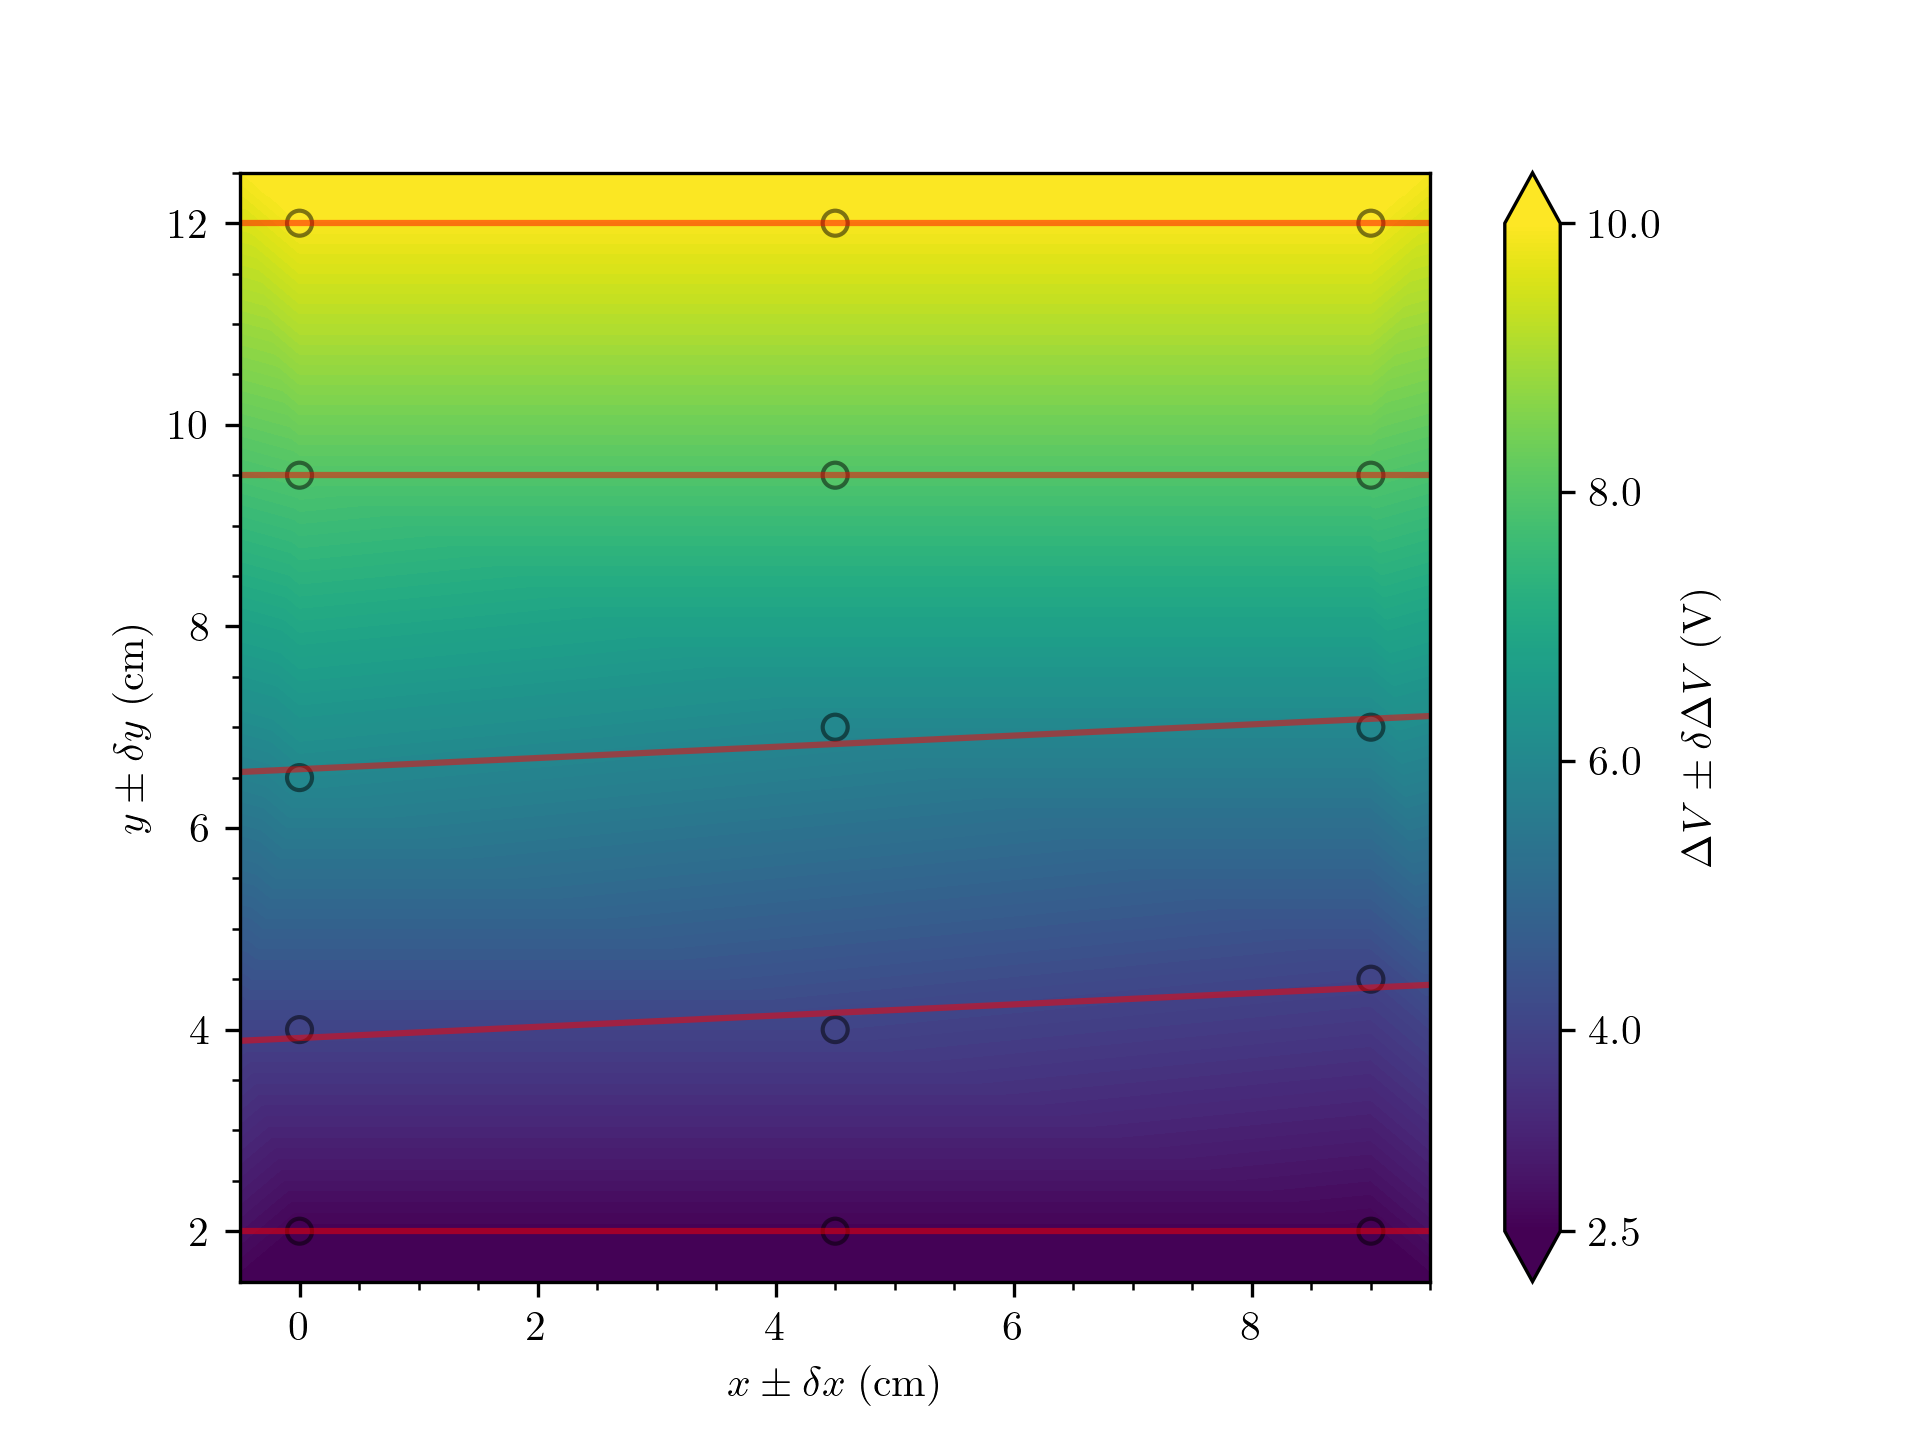
\includegraphics[scale=0.2]{plot1.png}
  \caption{Mediciones y Líneas Equipotenciales Parte A}
\label{fig:leqA}
\end{figure}

Observando las líneas equipotenciales es posible deducir que las mismas son paralelas si se dejan de lado errores experimentales.

Recordando que los vectores de campo eléctrico son perpendiculares a las líneas equipotenciales, podemos deducir que se encuentran dispuestos de la siguiente manera:

\phantom{x}

\begin{figure}[H]
\centerline{\hspace{0.5cm}\begin{tikzpicture}[scale=0.8]
	\begin{pgfonlayer}{nodelayer}
		\node [style=none] (25) at (1, 1) {};
		\node [style=none] (26) at (2, 1) {};
		\node [style=none] (27) at (3, 1) {};
		\node [style=none] (29) at (1, 0) {};
		\node [style=none] (30) at (2, 0) {};
		\node [style=none] (31) at (3, 0) {};
		\node [style=none] (35) at (3.5, 2.25) {$\vec{E_i}$};
		\node [style=none] (59) at (4.5, -0.25) {$\lambda_+$};
		\node [style=none] (70) at (0, 0) {};
		\node [style=none] (71) at (4, 0) {};
		\node [style=none] (92) at (1, 2) {};
		\node [style=none] (93) at (2, 2) {};
		\node [style=none] (94) at (3, 2) {};
		\node [style=none] (98) at (4.5, 2.75) {$\lambda_-$};
		\node [style=none] (99) at (0, 3) {};
		\node [style=none] (100) at (4, 3) {};
		\node [style=none] (101) at (0.25, 1.5) {};
		\node [style=none] (102) at (3.75, 1.5) {};
		\node [style=none] (111) at (5, 1.5) {$\Delta V = k_i$};
		\node [style=none] (112) at (1, 3) {};
		\node [style=none] (113) at (2, 3) {};
		\node [style=none] (114) at (3, 3) {};
	\end{pgfonlayer}
	\begin{pgfonlayer}{edgelayer}
		\draw [style=arrow] (29.center) to (25.center);
		\draw [style=arrow] (30.center) to (26.center);
		\draw [style=arrow] (31.center) to (27.center);
		\draw [style=line, bend right=360] (71.center) to (70.center);
		\draw [style=line, bend right=360] (100.center) to (99.center);
		\draw [style=dashy] (101.center) to (102.center);
		\draw [style=arrow] (27.center) to (94.center);
		\draw [style=arrow] (26.center) to (93.center);
		\draw [style=arrow] (25.center) to (92.center);
		\draw [style=arrow] (92.center) to (112.center);
		\draw [style=arrow] (93.center) to (113.center);
		\draw [style=arrow] (94.center) to (114.center);
	\end{pgfonlayer}
\end{tikzpicture}}
\caption{Representación Estimada del Campo Eléctrico Parte A}
\label{fig:repA}
\end{figure}

Esta disposición coincide con la representación planteada para el campo eléctrico producido por una línea cargada en el marco teórico.

En cuanto a la magnitud del campo eléctrico en los distintos puntos del plano, es posible hallarla utilizando la ecuación \ref{eq:MagE}, que vincula la magnitud del vector campo eléctrico con el gradiente de potencial. Si graficamos esta información de forma similar a la ya utilizada el resultado es este:

\begin{figure}[H]
  \hspace{-0.1cm}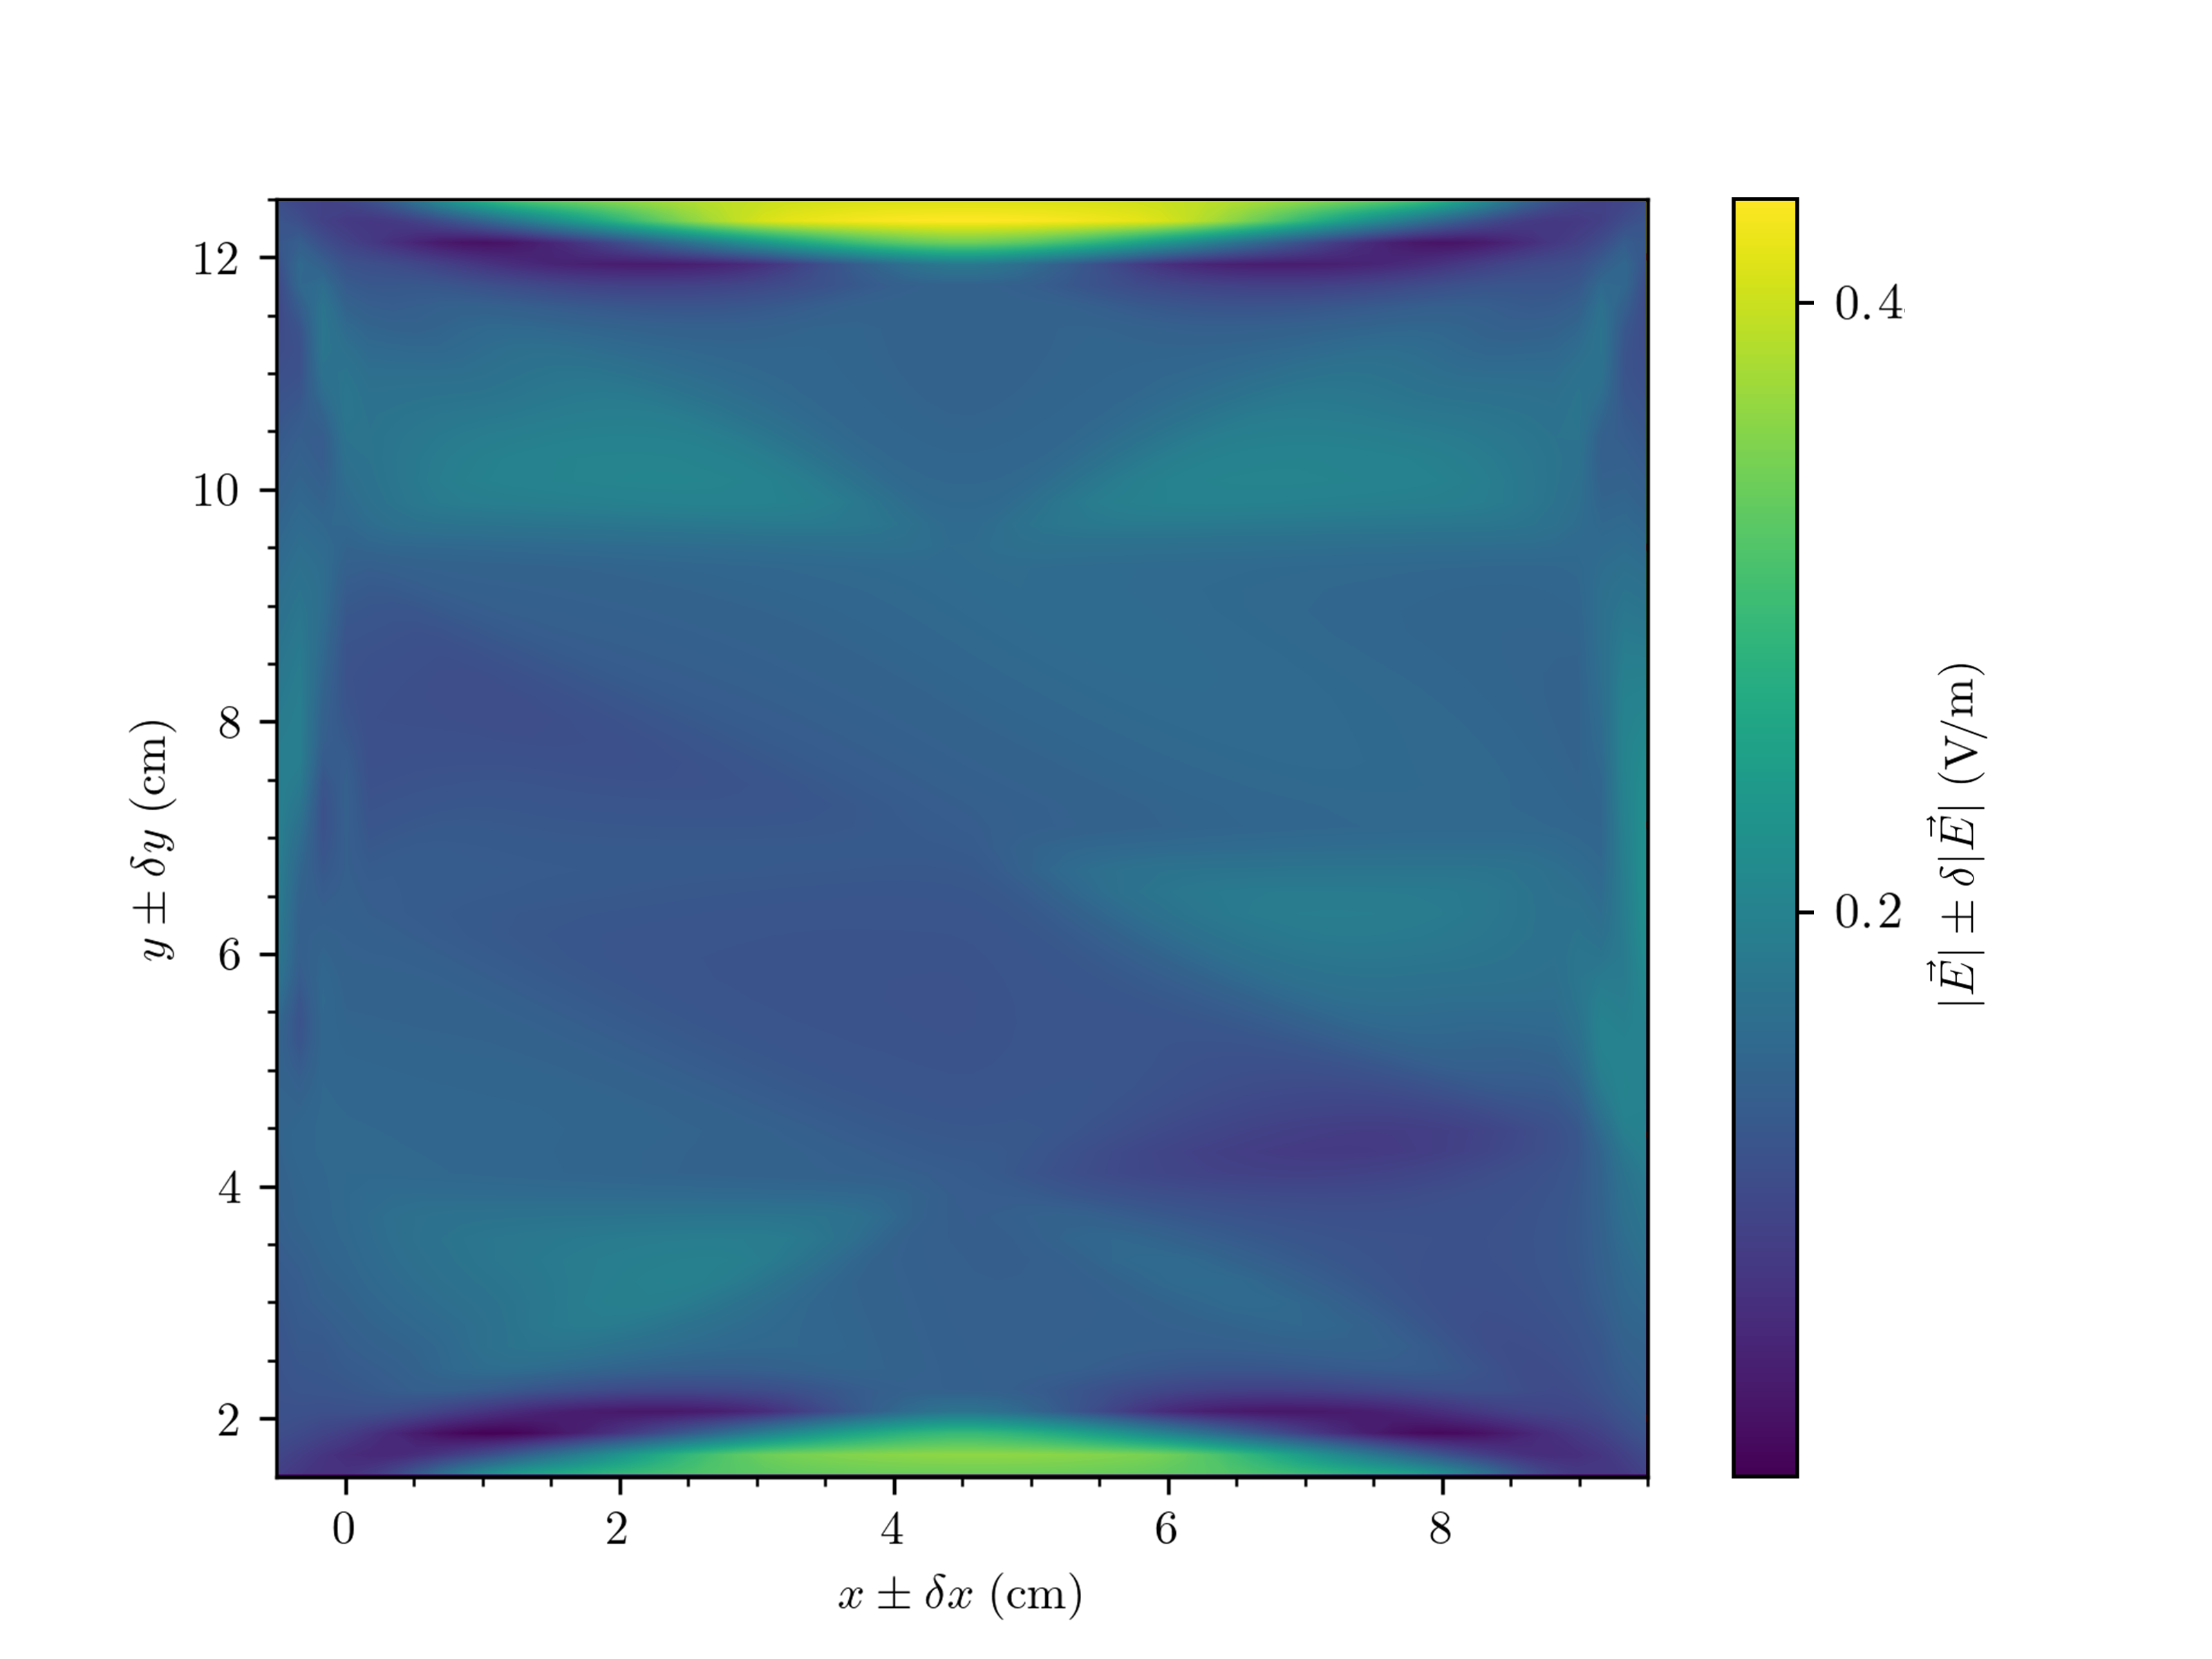
\includegraphics[scale=0.12]{plot4.png}
  \caption{Magnitud de Campo Eléctrico Parte A}
\end{figure}

Esto coincide con el modelo teórico, donde se plantea que la magnitud del campo eléctrico es constante entre dos placas paralelas con cargas opuestas, siempre y cuando se considere que la información fuera del entorno entre $\Delta V = 10.0 \;\text{V}$ o ${y} = 12$ cm, y $\Delta V = 2.5$ V o $y = 2$ cm, no fue medida (véase la figura \ref{fig:leqA}), y por tanto esta información no corresponde al modelo.

De igual forma fueron representadas las mediciones obtenidas en la parte B. En este caso, las líneas equipotenciales correspondientes fueron obtenidas realizando interpolaciones cúbicas de los puntos pertenecientes.

\vfill

\vspace*{-2cm}

\begin{figure}[H]
  \hspace{-0.1cm}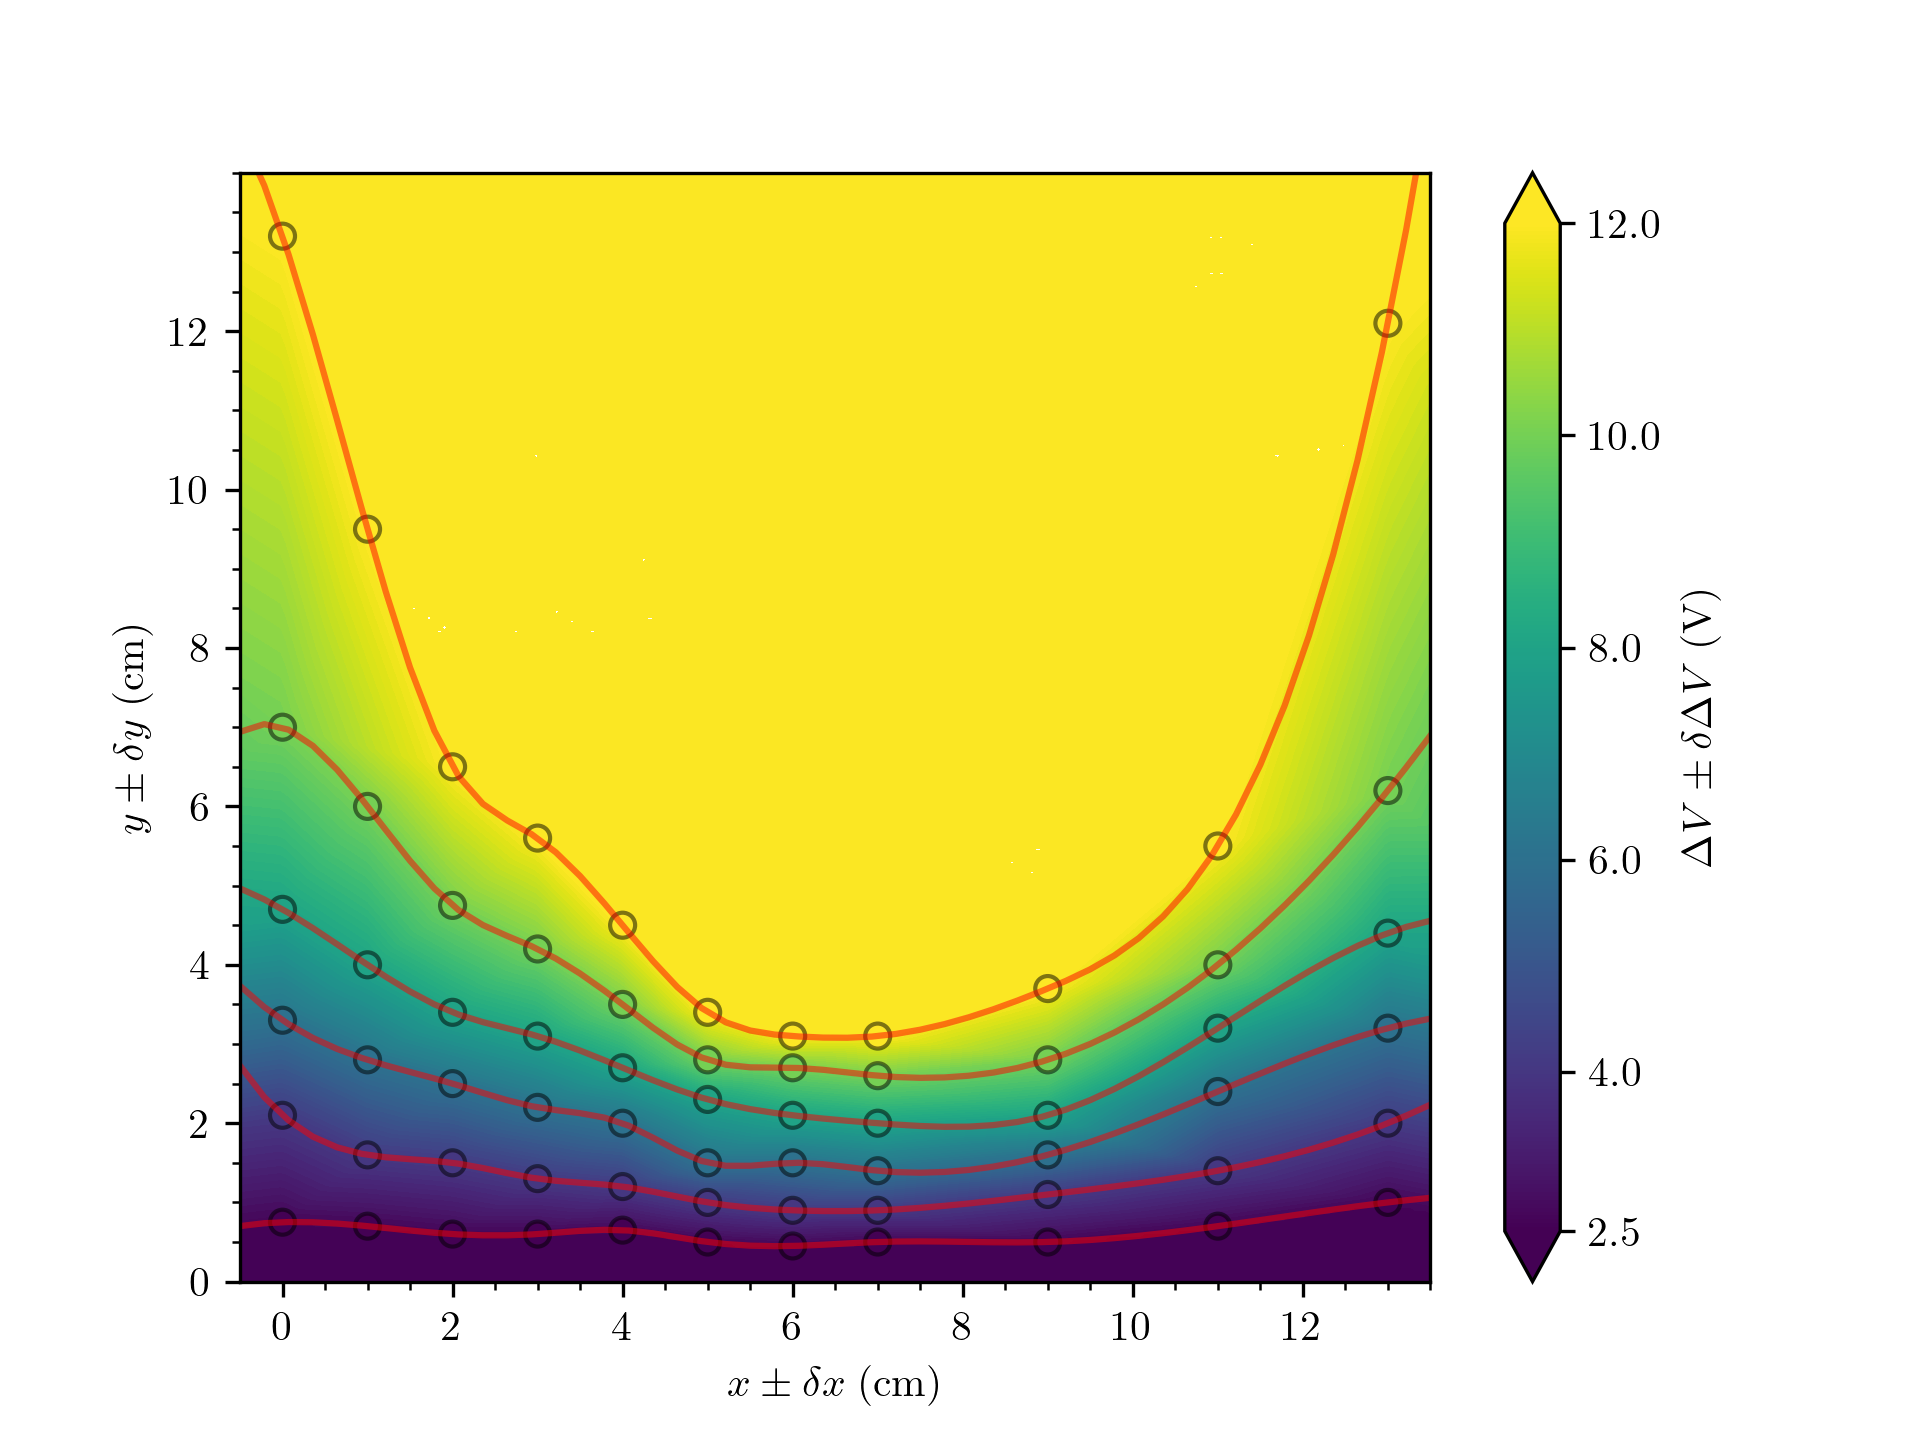
\includegraphics[scale=0.2]{plot2.png}
  \label{fig:leqB}
  \caption{Mediciones y Líneas Equipotenciales Parte B}
\end{figure}

En este caso es posible ver como las líneas equipotenciales se ``comprimen'' entre el cilindro y la placa cargada. Esto significa que el gradiente de potencial eléctrico es mayor para los valores de $x$ centrales, más cercanos al cilindro conductor, que para los valores de $x$ extremos.

Si representamos los vectores de campo eléctrico de igual forma que en la figura \ref{fig:repA}, perpendiculares a las líneas equipotenciales, la disposición se asemeja a la siguiente:

\phantom{x}

\begin{figure}[H]
\centerline{\hspace{1cm}\begin{tikzpicture}[scale=0.4]
	\begin{pgfonlayer}{nodelayer}
		\node [style=none] (3) at (1.5, 0) {};
		\node [style=none] (4) at (4.5, 0) {};
		\node [style=none] (5) at (7.5, 0) {};
		\node [style=none] (6) at (8, 5) {$\vec{E_i}$};
		\node [style=none] (7) at (10, -0.5) {$\lambda_+$};
		\node [style=none] (8) at (0, 0) {};
		\node [style=none] (9) at (9, 0) {};
		\node [style=none] (13) at (10, 5.5) {$\lambda_-$};
		\node [style=none] (14) at (0, 6) {};
		\node [style=none] (15) at (9, 6) {};
		\node [style=none] (18) at (11, 4) {$\Delta V = k_i$};
		\node [style=none] (19) at (3, 6) {};
		\node [style=none] (20) at (4.5, 6) {};
		\node [style=none] (21) at (6, 6) {};
		\node [style=none] (22) at (4.5, 4) {};
		\node [style=none] (23) at (3.5, 3) {};
		\node [style=none] (24) at (4.5, 2) {};
		\node [style=none] (25) at (5.5, 3) {};
		\node [style=none] (26) at (3.75, 2.25) {};
		\node [style=none] (27) at (5.25, 2.25) {};
		\node [style=none] (28) at (5.25, 3.75) {};
		\node [style=none] (29) at (3.75, 3.75) {};
		\node [style=none] (30) at (3, 0) {};
		\node [style=none] (31) at (6, 0) {};
		\node [style=none] (32) at (1.5, 6) {};
		\node [style=none] (33) at (7.5, 6) {};
		\node [style=none] (43) at (0, 4) {};
		\node [style=none] (44) at (1.25, 3.75) {};
		\node [style=none] (45) at (2, 2.75) {};
		\node [style=none] (46) at (3, 1.75) {};
		\node [style=none] (47) at (4.5, 1.25) {};
		\node [style=none] (48) at (6, 1.75) {};
		\node [style=none] (49) at (7, 2.75) {};
		\node [style=none] (50) at (7.75, 3.75) {};
		\node [style=none] (51) at (9, 4) {};
	\end{pgfonlayer}
	\begin{pgfonlayer}{edgelayer}
		\draw [style=line, bend right=360] (9.center) to (8.center);
		\draw [style=line, bend right=360] (15.center) to (14.center);
		\draw [style=someshape, bend left=45] (23.center) to (22.center);
		\draw [style=someshape, bend left=45] (22.center) to (25.center);
		\draw [style=someshape, bend left=45] (25.center) to (24.center);
		\draw [style=someshape, bend right=315] (24.center) to (23.center);
		\draw [style=arrow, bend right=15] (31.center) to (27.center);
		\draw [style=arrow] (4.center) to (24.center);
		\draw [style=arrow, bend left=15] (30.center) to (26.center);
		\draw [style=arrow, bend left] (3.center) to (23.center);
		\draw [style=arrow, bend right] (5.center) to (25.center);
		\draw [style=arrow, bend left] (23.center) to (32.center);
		\draw [style=arrow, bend left=15] (29.center) to (19.center);
		\draw [style=arrow] (22.center) to (20.center);
		\draw [style=arrow, bend right=15] (28.center) to (21.center);
		\draw [style=arrow, bend right] (25.center) to (33.center);
    \draw [style=dashy, rounded corners=3mm] (43.center)--(44.center)--(45.center)--(46.center)--(47.center)--(48.center)--(49.center)--(50.center)--(51.center);
	\end{pgfonlayer}
\end{tikzpicture}}
\caption{Representación Estimada del Campo Eléctrico Parte B}
\label{fig:repB}
\end{figure}

Esta disposición de los vectores de campo se asemeja con el resultado teórico de colocar un conductor sin carga en un campo eléctrico uniforme.

Además de verificar la disposición, podemos nuevamente analizar la magnitud del campo eléctrico en el plano. Recurriendo nuevamente a la ecuación \ref{eq:MagE}, obtenemos el siguiente gráfico:

\begin{figure}[H]
  \hspace{-0.1cm}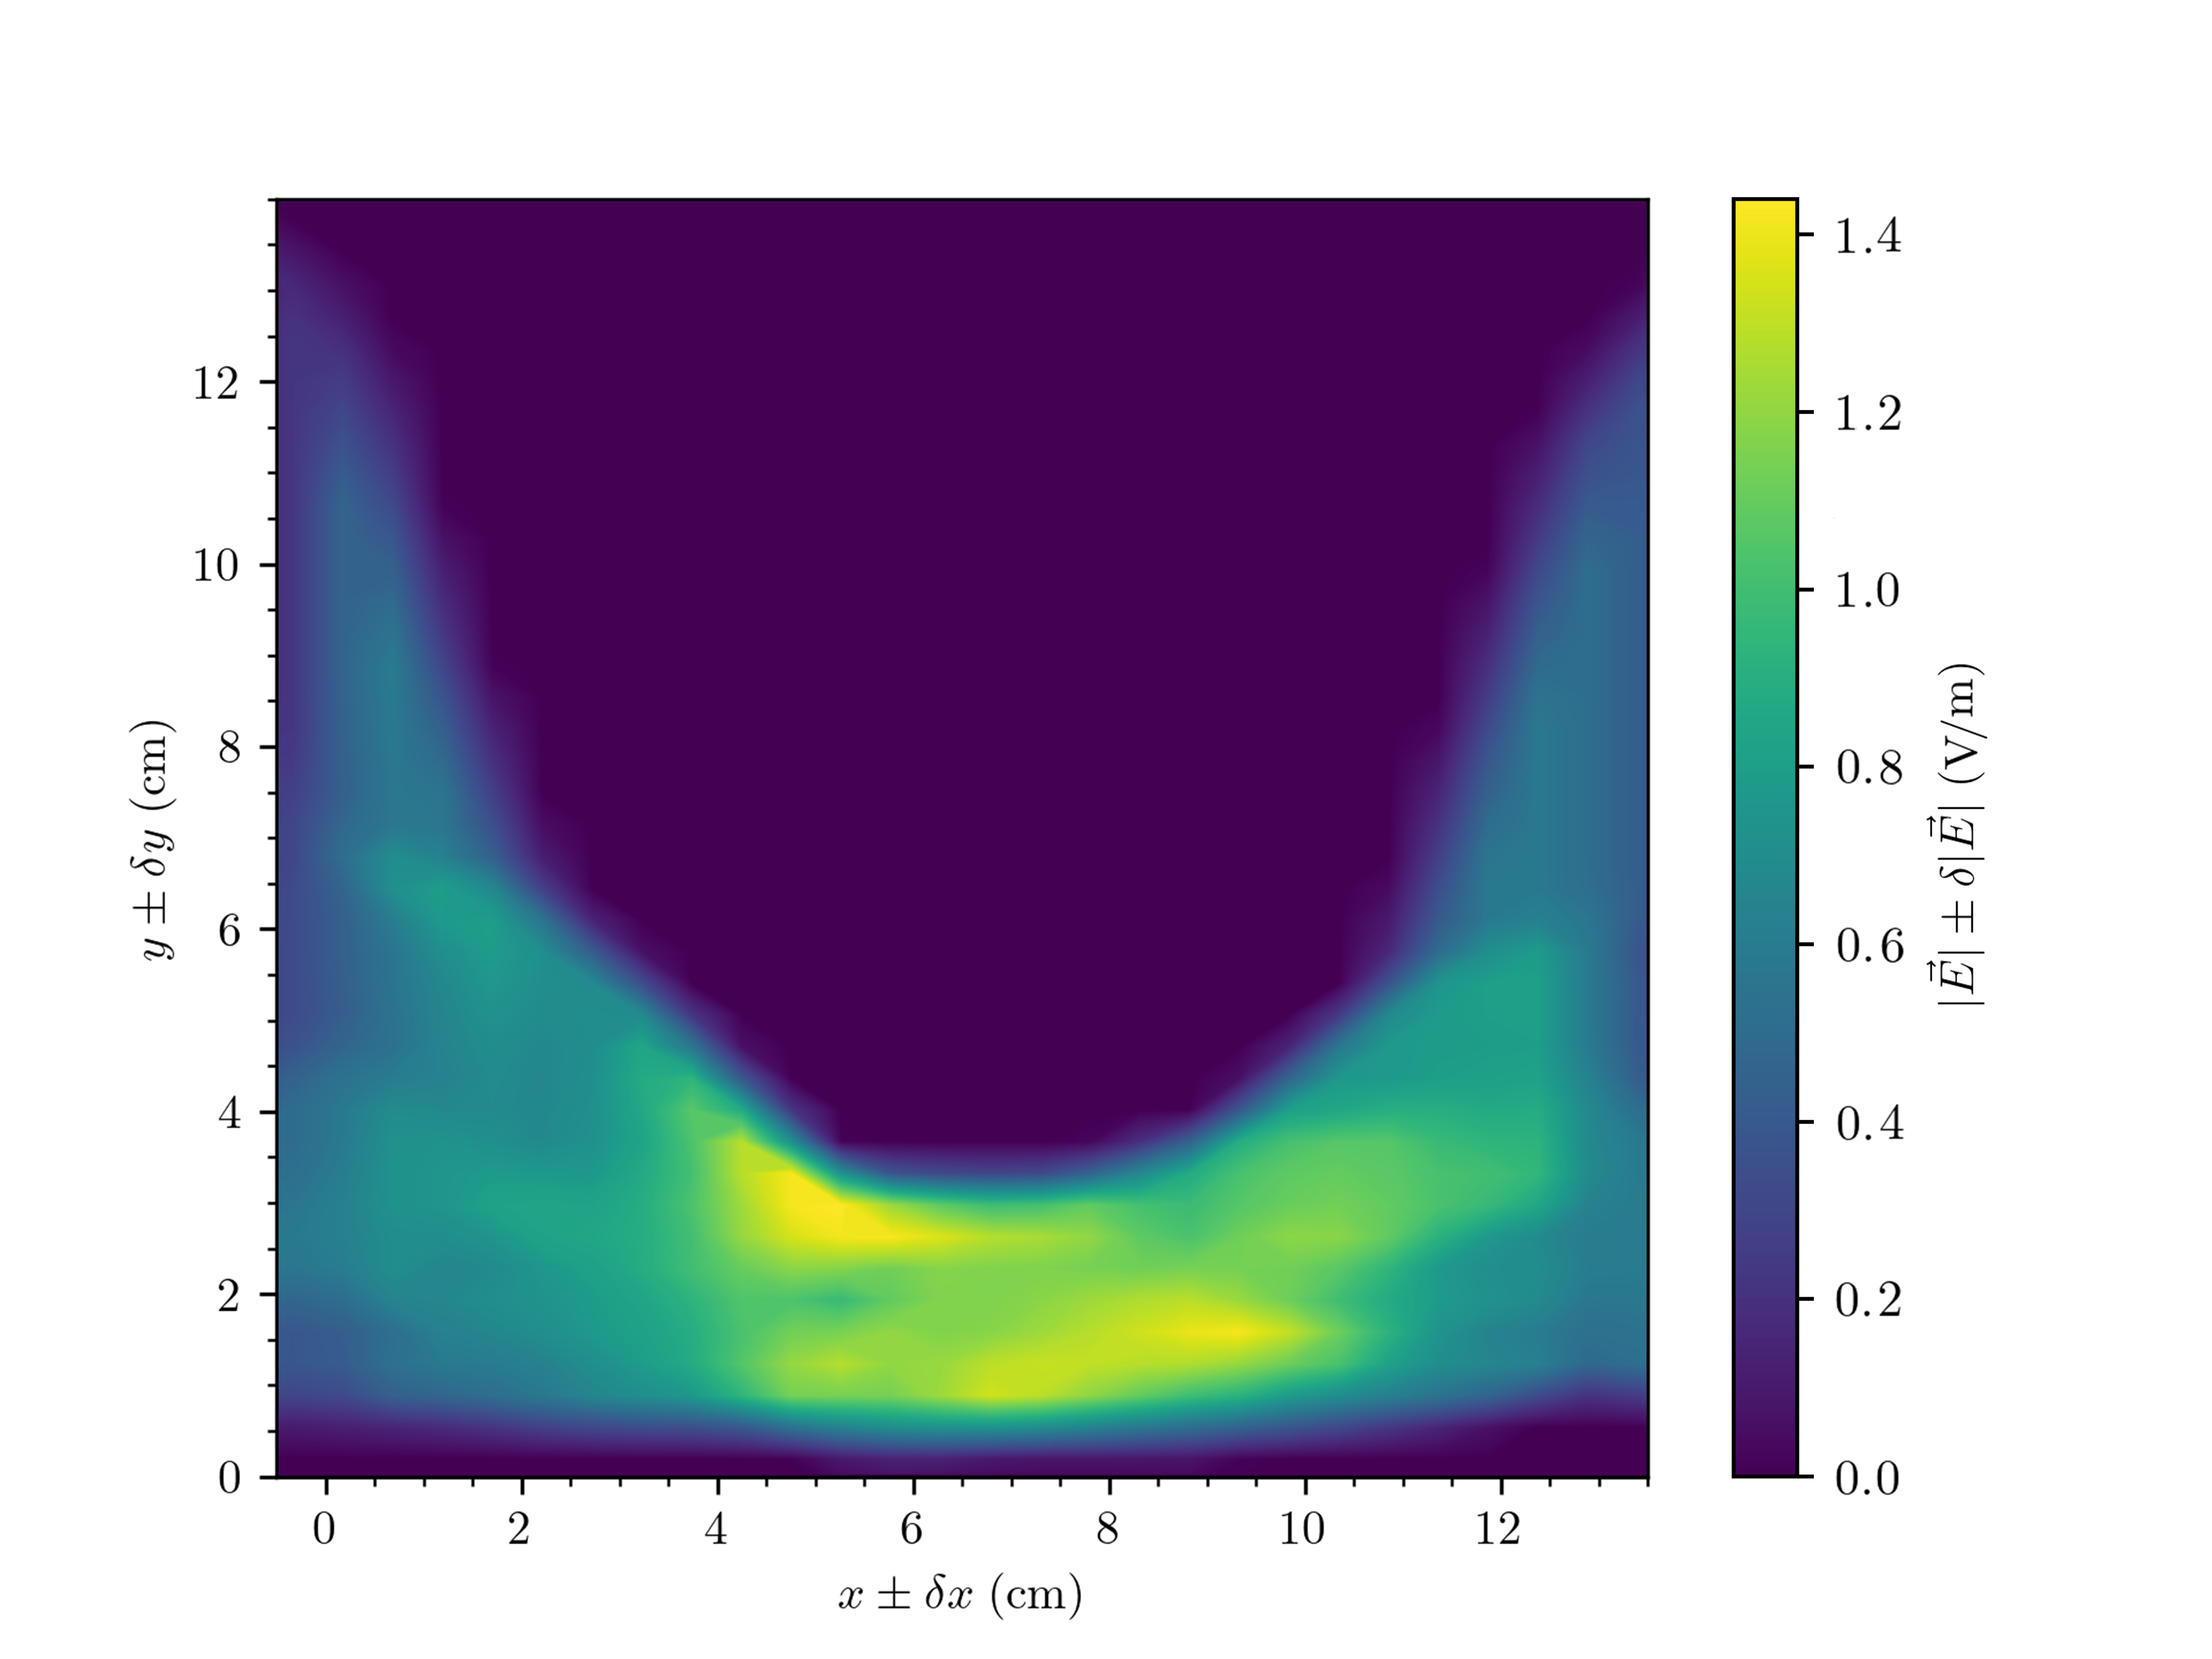
\includegraphics[scale=0.12]{plot3.png}
  \caption{Magnitud de Campo Eléctrico Parte B}
\end{figure}

Considerando que no fueron tomadas medidas por encima de la línea equipotencial $\Delta V = 12.0$ V, ni debajo de $\Delta V = 2.5$ V, (véase la figura 4) los datos en estos entornos son no observados. Para la información del entorno observado, este gráfico es coherente con lo esperado segun el diagrama anterior, pues más cerca del centro existe mayor densidad de líneas de campo.

\section{Conclusiones}

Recopilando la información, concluimos que, en primer lugar, es posible determinar la disposición y magnitudes de los vectores de campo eléctrico entre dos placas utilizando las líneas equipotenciales. 

También se concluye que en la presencia de dos placas cargadas las líneas equipotenciales son paralelas a las placas y los vectores de campo eléctrico son perpendiculares a estas. Otra conclusión que con la presencia de un cuerpo conductor en un campo eléctrico uniforme, las líneas equipotenciales se deforman alrededor del cuerpo y los vectores de campo lo hacen hacia el mismo.

Sobre la magnitud de campo eléctrico, concluímos que estando un cuerpo conductor a menor distancia del origen del campo, mayor es la magnitud del campo eléctrico entre estos.

\section{Bibliografía}

\begin{enumerate}
    \item Bonda, E. (2010). Electromagnetismo. El Mendrugo.
    \item Anderson, P. W. P. [@yoprofmatt]. (2016, octubre 9). How to get electric field from electric potential. Youtube.\\https://www.youtube.com/watch?v=vmW7h5YgZL8

\end{enumerate}

\end{document}